% Chapter Template
\chapter{Theoretical study of Turing patterns }
\section{Synopsis}
Usually when we study pattern formation, we look for Turing patterns.
First we do so analytically (faster) and then we do it numerically (we can see shape and evolution).
In this chapter, we first study the relationship between the dispersion relation and the numerical results in Turing patterns.
This includes understanding how to predict wavelength, convergence time and even pattern shape from the dispersion.
Then we explore how linear stability analysis might not be a good predictor of pattern formation.
For example, how multistability can break linear stability analysis predictions and how other types of dispersion relation profiles or instabilities which are not classical Turing can generate stationary spatial patterns.
Finally, we explore numerically how these patterns behave when realistic biological systems from our experimental setup are introduced, including open boundaries or growth.
\section{Motivation and open questions}
%todo comment on much work done analytically but reallity is numerical. We miss links. Also we lack reality in terms of growh and other important realistic phenomena




\section{Pattern information in the dispersion relation of Turing instabilities}

\subsection{The dispersion relation}
%intro to dispersion relation

\subsection{Infering wavelength and convergence time from dispersion relation}

\begin{figure}[h] % h! is a placement specifier; it tries to place the image here.
    \centering
    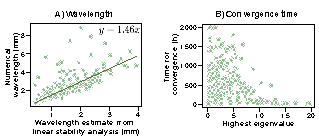
\includegraphics[width=1\textwidth]{chapters/Chapter 1/dispersion_to_wavelength_convergence} % The name of your image file; assumes it's in the same directory as your .tex file
    \caption{A sample caption for the image.}
    \label{fig:dispersion_to_wavelength_convergence} % A label for referencing this figure later in the document
\end{figure}


\subsection{Dispersion to pattern}
dispersion to pattern
\begin{figure}[h] % h! is a placement specifier; it tries to place the image here.
    \centering
    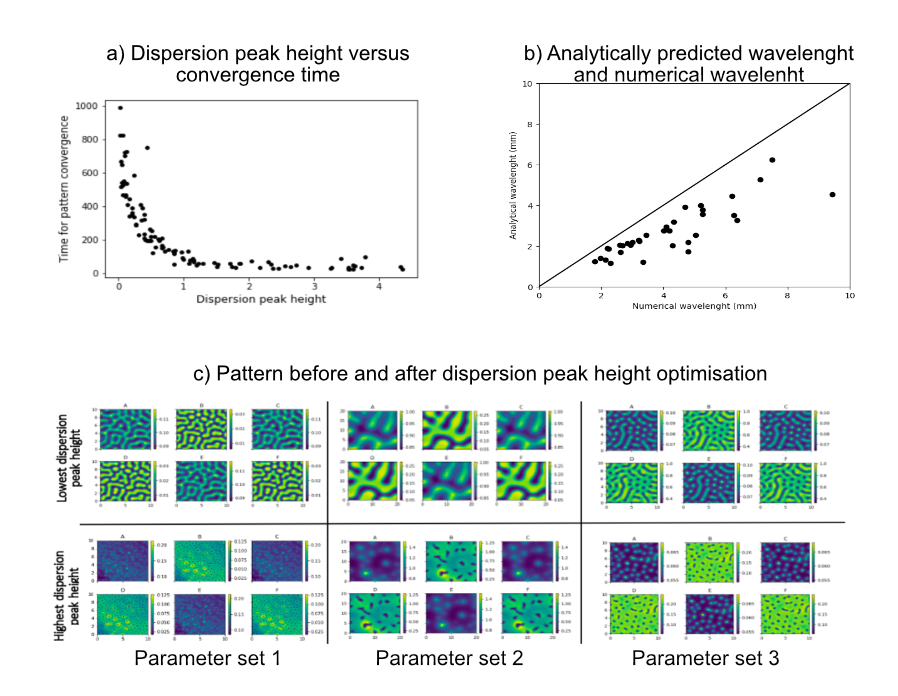
\includegraphics[width=1\textwidth]{chapters/Chapter 1/dispersion_to_shape} % The name of your image file; assumes it's in the same directory as your .tex file
    \caption{A sample caption for the image.}
    \label{fig:dispersion_to_shape} % A label for referencing this figure later in the document
\end{figure}



\section{Breaking linear stability analysis predictions}

\subsection{multistability in Turing}
multistaabilityaa
%todo make subfigures bigger
%todo pass all images into pdf

\begin{adjustbox}{width=1.4\textwidth,center}
\begin{figure}
    \centering
    \subfigure[]{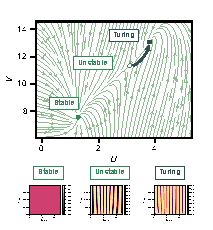
\includegraphics[width=0.45\linewidth]{chapters/Chapter 1/multistability1}}
    \subfigure[]{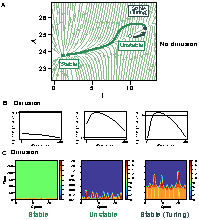
\includegraphics[width=0.45\linewidth]{chapters/Chapter 1/multistability2}}
    \subfigure[]{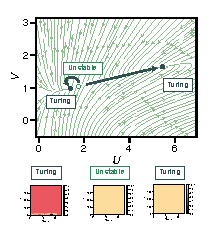
\includegraphics[width=0.45\linewidth]{chapters/Chapter 1/multistability3}}
    \subfigure[]{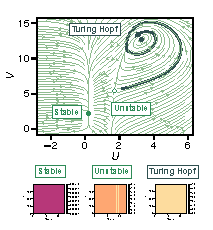
\includegraphics[width=0.45\linewidth]{chapters/Chapter 1/multistability4}}
    \subfigure[]{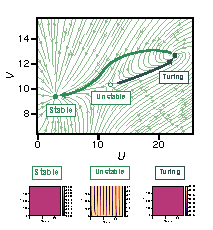
\includegraphics[width=0.45\linewidth]{chapters/Chapter 1/multistability5}}
    \subfigure[]{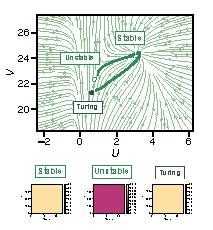
\includegraphics[width=0.45\linewidth]{chapters/Chapter 1/multistability6}}

    \caption{(a) blah (b) blah (c) blah (d) blah}
    \label{fig:foobar}
\end{figure}
\end{adjustbox}


\subsection{Analytical to numerical: Other types of dispersion relation, and other types of patterns}
 %todo . They also identify examples of non-stationary spatial patterns, when the eigenvalue corresponding to a critical wave number has non-zero imaginary part.Deutsch, A., Dormann, S., et al., 2005. Cellular automaton modeling of biological pattern formation. Springer.

%todo look at pitchfork and transcritical

\section{Introducing realistic biological phenomena}
\subsection{No growth to open boundaries}
\subsection{Open boundaries to growth}


\section{methods}
\subsection{lsa}

%todo look at leyshon paper for lsa explanation
